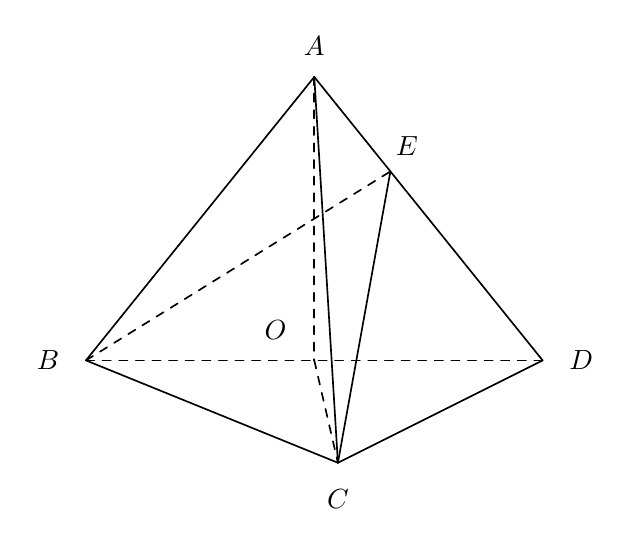
\begin{tikzpicture}[line width=0.6pt,line join=round,line cap=round]
\coordinate (A) at (0,4.2);
\coordinate (B) at (-2.9,0.6);
\coordinate (D) at (2.9,0.6);
\coordinate (O) at (0,0.6);
\coordinate (C) at (0.3,-0.7);
\coordinate (E) at (0.9666666667,3.0000000000);
% base BD (hidden, O on it)
\draw[dashed] (B) -- (O) -- (D);
% vertical AO (hidden) and OC (hidden)
\draw[dashed] (A) -- (O);
\draw[dashed] (O) -- (C);
% diagonal BE (hidden)
\draw[dashed] (B) -- (E);
% solid lateral and base edges
\draw (A) -- (B);
\draw (A) -- (D);
\draw (B) -- (C);
\draw (D) -- (C);
% solid interior segments AC and EC
\draw (A) -- (C);
\draw (E) -- (C);
% labels with clearance
\node[above=4pt] at (A) {$A$};
\node[left=6pt] at (B) {$B$};
\node[right=6pt] at (D) {$D$};
\node[below=6pt] at (C) {$C$};
\node[left=7pt,above=2pt,xshift=-7pt,yshift=2pt] at (O) {$O$};
\node[right=6pt,above=2pt] at (E) {$E$};
\end{tikzpicture}
